% Appendix Template

\chapter{Other Solutions for MLCA} % Main appendix title

\section{2 classes in day level}

\label{AppendixC} % Change X to a consecutive letter; for referencing this appendix elsewhere, use \ref{AppendixX}

\begin{figure}[H]
	%\vspace*{13cm}
	\centering
	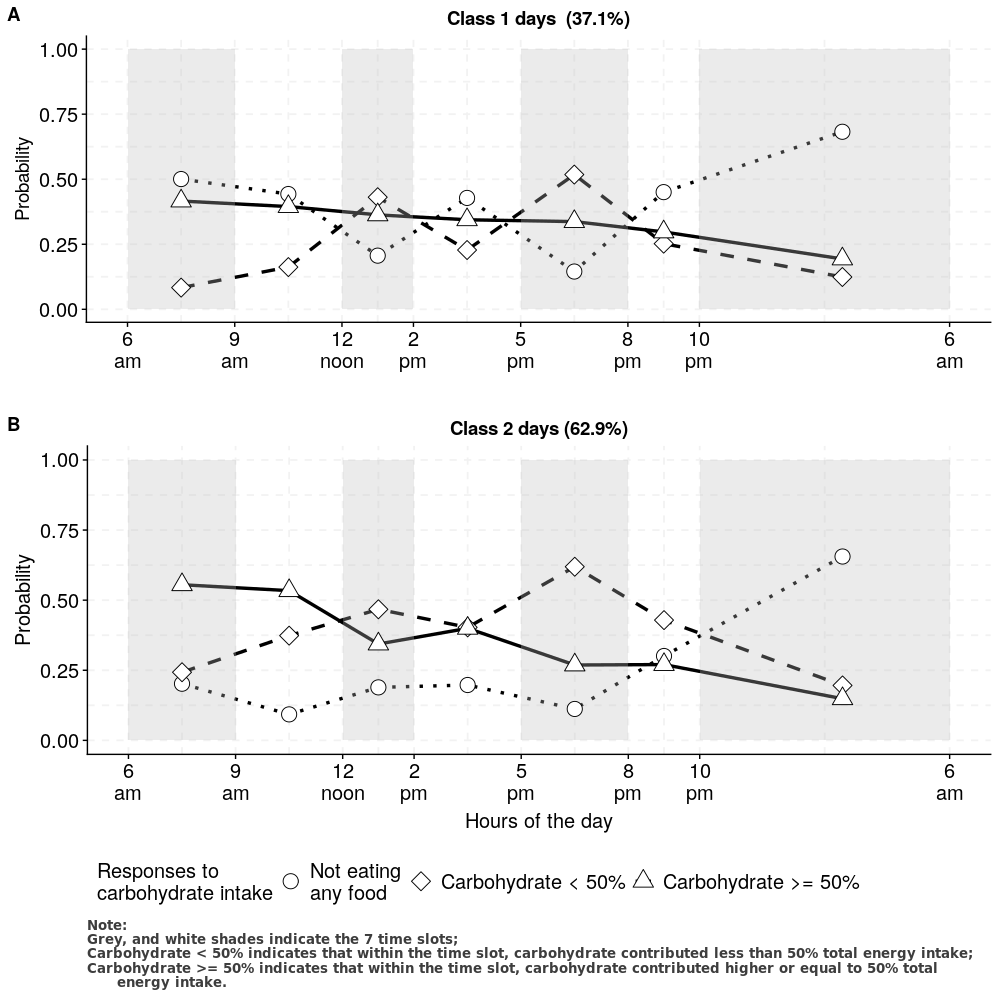
\includegraphics{Figures/CW2level1.png}
	\decoRule
	\caption[2 Classes solution in Day level]{2 Classes solution in Day level.}
	\label{fig:diary1}
\end{figure}



\begin{figure}[H]
	%\vspace*{13cm}
	\centering
	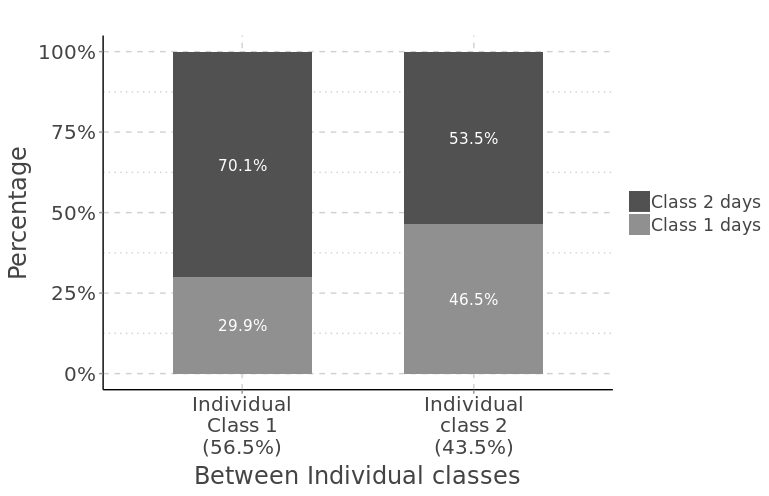
\includegraphics[width=13cm]{Figures/CW2CB2.png}
	\decoRule
	\caption[Multilevel Latent Class Solution (2 $\times$ 2).]{Multilevel Latent Class Solution, 2 classes in day level, 2 classes in individual level.}
	\label{fig:diary1}
\end{figure}




\begin{figure}[H]
	%\vspace*{13cm}
	\centering
	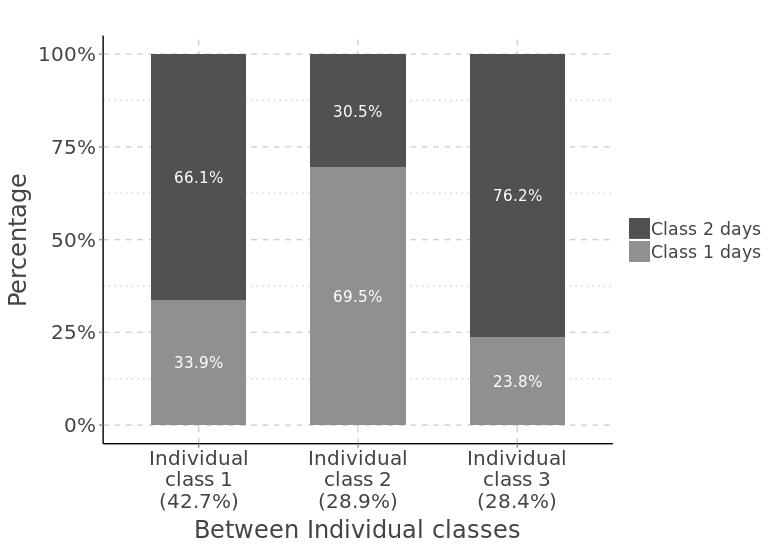
\includegraphics[width=13cm]{Figures/CW2CB3.png}
	\decoRule
	\caption[Multilevel Latent Class Solution (2 $\times$ 3).]{Multilevel Latent Class Solution, 2 classes in day level, 3 classes in individual level.}
	\label{fig:diary1}
\end{figure}


\begin{figure}[H]
	%\vspace*{13cm}
	\centering
	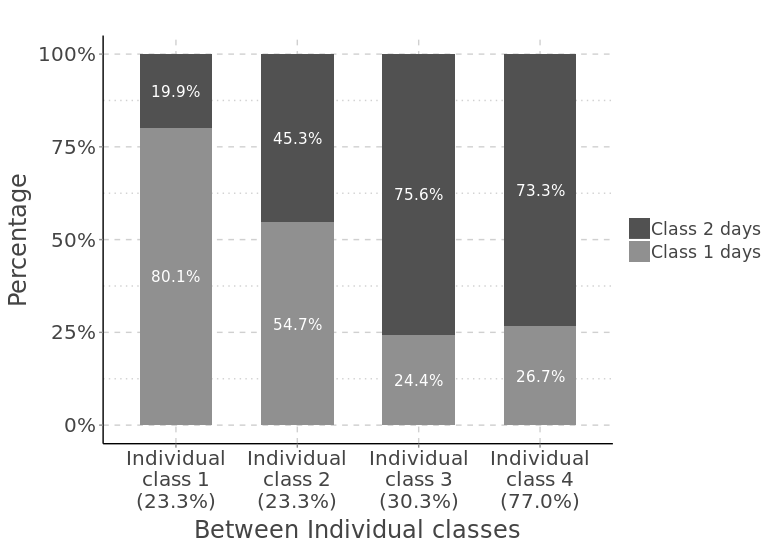
\includegraphics[width=13cm]{Figures/CW2CB4.png}
	\decoRule
	\caption[Multilevel Latent Class Solution (2 $\times$ 4).]{Multilevel Latent Class Solution, 2 classes in day level, 4 classes in individual level.}
	\label{fig:diary1}
\end{figure}

\section{3 classes in day level, 4 classes in individual level}\vspace{-0.3cm}

\begin{figure}[H]
	%\vspace*{13cm}
	\centering
	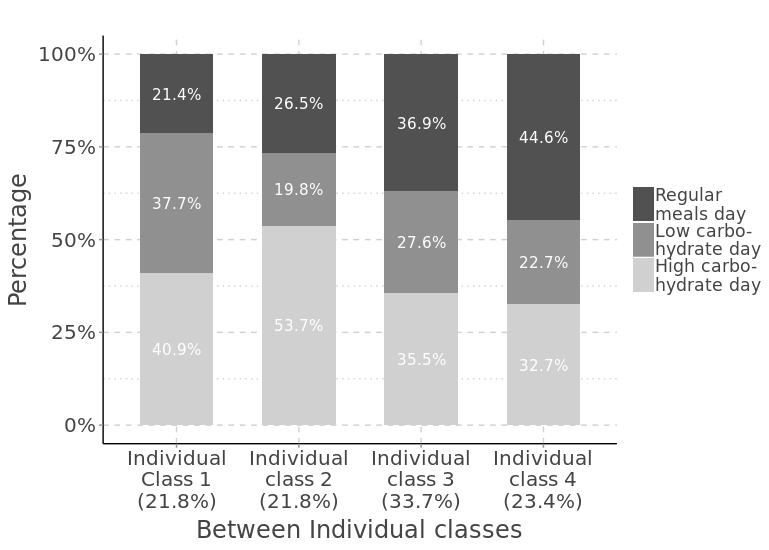
\includegraphics[width=13cm]{Figures/CW3CB4.png}
	\decoRule
	\caption[Multilevel Latent Class Solution (3 $\times$ 4).]{Multilevel Latent Class Solution, 3 classes in day level, 4 classes in individual level.}
	\label{fig:diary1}
\end{figure}


\section{4 classes in day level}

\begin{figure}[H]
	%\vspace*{13cm}
	\centering
	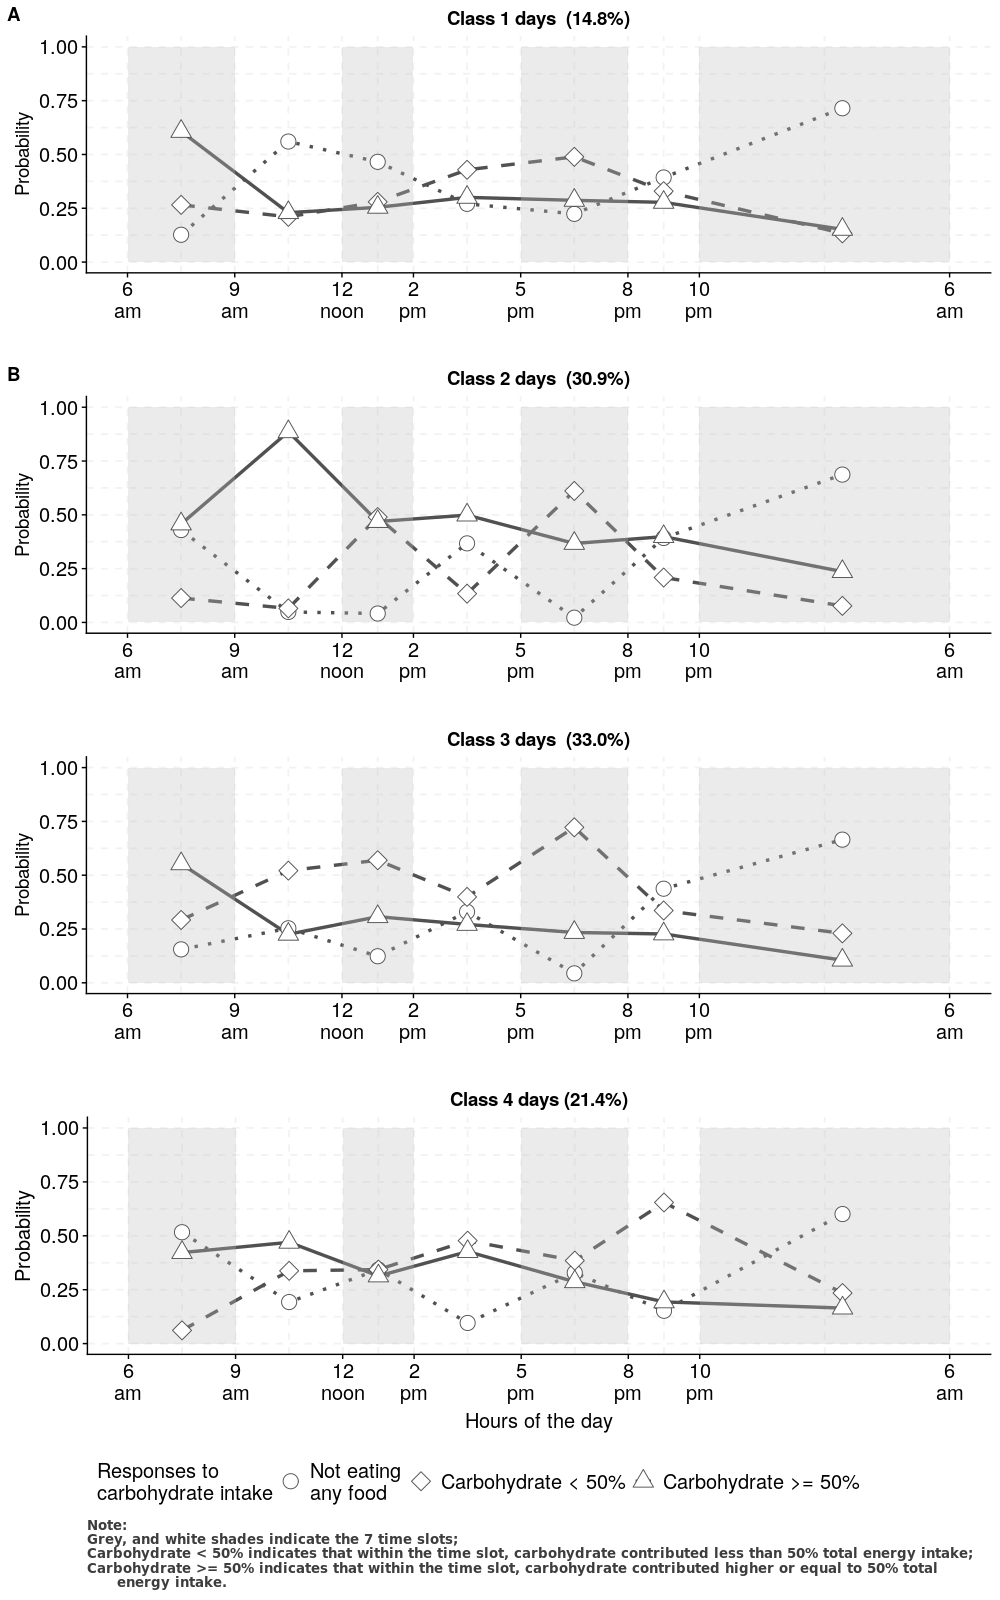
\includegraphics[width=15cm]{Figures/CW4level1.png}
	\decoRule
	\caption[2 Classes Solution in Day level]{4 Classes Solution in Day level.}
	\label{fig:diary1}
\end{figure}

